\documentclass[tikz,border=8pt]{standalone}
\usetikzlibrary{arrows.meta,positioning,calc}
\makeatletter
\AtBeginDocument{\global\let\pgf@selectfontorig\relax}
\makeatother

\tikzset{
  nodebox/.style={draw=black, rounded corners=4pt, very thick, fill=gray!4,
    minimum width=10mm, minimum height=7mm, align=center, inner sep=2pt},
  initial/.style={-Latex, very thick},
  edge/.style={-Latex, thick, shorten >=1pt, shorten <=1pt},
  labelbox/.style={fill=white, inner sep=1.2pt, font=\scriptsize},
  aptxt/.style={font=\scriptsize, text=gray!65!black, anchor=north east},
}

\newcommand{\initarrow}[2]{\draw[initial] #1 -- (#2);}
\newcommand{\statelabel}[2]{\node[aptxt] at ($(#1.south east)+(0.02,-0.05)$) {#2};}

\begin{document}
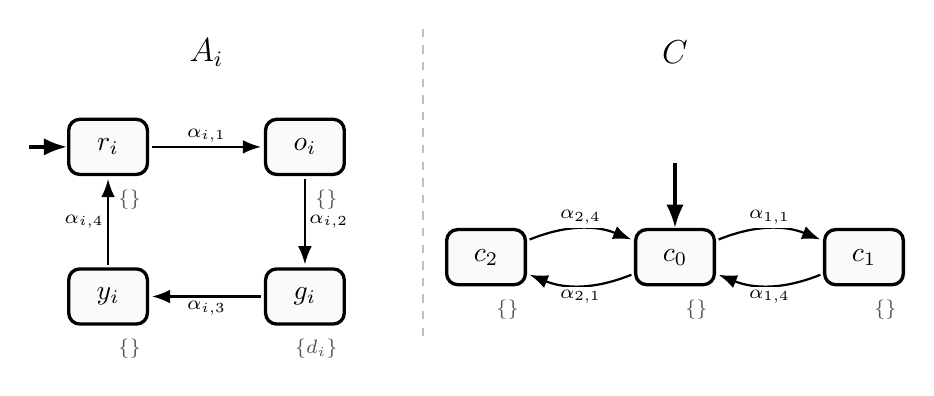
\begin{tikzpicture}[scale=1, transform shape]

  %% ---- A_i (left panel) ----
  \begin{scope}[shift={(0,0)}]
    \node[font=\bfseries\large] at (1.25, 1.2) {$A_i$};

    \node[nodebox] (r) at (0,    0  ) {$r_i$};
    \node[nodebox] (o) at (2.5,  0  ) {$o_i$};
    \node[nodebox] (g) at (2.5, -1.9) {$g_i$};
    \node[nodebox] (y) at (0,   -1.9) {$y_i$};

    \statelabel{r}{$\{\}$};
    \statelabel{o}{$\{\}$};
    \statelabel{g}{$\{d_i\}$};
    \statelabel{y}{$\{\}$};

    \initarrow{(-1.0, 0)}{r.west}

    \draw[edge] (r) -- node[labelbox, above] {$\alpha_{i,1}$} (o);
    \draw[edge] (o) -- node[labelbox, right] {$\alpha_{i,2}$} (g);
    \draw[edge] (g) -- node[labelbox, below] {$\alpha_{i,3}$} (y);
    \draw[edge] (y) -- node[labelbox, left]  {$\alpha_{i,4}$} (r);
  \end{scope}

  %% ---- Vertical divider ----
  \draw[dashed, gray!50, thick] (4.0, 1.5) -- (4.0, -2.4);

  %% ---- Controller C -- Safety variant (right panel) ----
  %% Centers: A_i center = y=-0.95; C nodes at y=0, init arrow top y=1.2 -> center~0.45
  %% Shift C down by 0.95+0.45=1.40 to align centers
  \begin{scope}[shift={(7.2,-1.40)}]
    \node[font=\bfseries\large] at (0, 2.6) {$C$};

    \node[nodebox] (b0) at ( 0,    0) {$c_0$};
    \node[nodebox] (b1) at ( 2.4,  0) {$c_1$};
    \node[nodebox] (b2) at (-2.4,  0) {$c_2$};

    \statelabel{b0}{$\{\}$};
    \statelabel{b1}{$\{\}$};
    \statelabel{b2}{$\{\}$};

    \initarrow{(0, 1.2)}{b0.north}

    \draw[edge, bend left=22] (b0) to node[labelbox, above] {$\alpha_{1,1}$} (b1);
    \draw[edge, bend left=22] (b1) to node[labelbox, below] {$\alpha_{1,4}$} (b0);
    \draw[edge, bend left=22] (b0) to node[labelbox, below] {$\alpha_{2,1}$} (b2);
    \draw[edge, bend left=22] (b2) to node[labelbox, above] {$\alpha_{2,4}$} (b0);
  \end{scope}

\end{tikzpicture}
\end{document}

    \statelabel{y}{$\{\}$};

    \initarrow{(-1.0, 0)}{r.west}

    \draw[edge] (r) -- node[labelbox, above] {$\alpha_{i,1}$} (o);
    \draw[edge] (o) -- node[labelbox, right] {$\alpha_{i,2}$} (g);
    \draw[edge] (g) -- node[labelbox, below] {$\alpha_{i,3}$} (y);
    \draw[edge] (y) -- node[labelbox, left]  {$\alpha_{i,4}$} (r);
  \end{scope}

  %% ---- Controller C -- Safety variant (right panel) ----
  %% A_i center ≈ y=-0.95; C horizontal bar center = y=0 before shift
  %% shift down by 0.95 to align centers
  \begin{scope}[shift={(6.5,-0.95)}]
    \node[font=\bfseries\large] at (0, 2.0) {$C$};

    \node[nodebox] (b0) at ( 0,    0) {$c_0$};
    \node[nodebox] (b1) at ( 2.4,  0) {$c_1$};
    \node[nodebox] (b2) at (-2.4,  0) {$c_2$};

    \statelabel{b0}{$\{\}$};
    \statelabel{b1}{$\{\}$};
    \statelabel{b2}{$\{\}$};

    \initarrow{(0, 1.2)}{b0.north}

    \draw[edge, bend left=22] (b0) to node[labelbox, above] {$\alpha_{1,1}$} (b1);
    \draw[edge, bend left=22] (b1) to node[labelbox, below] {$\alpha_{1,4}$} (b0);
    \draw[edge, bend left=22] (b0) to node[labelbox, below] {$\alpha_{2,1}$} (b2);
    \draw[edge, bend left=22] (b2) to node[labelbox, above] {$\alpha_{2,4}$} (b0);
  \end{scope}

\end{tikzpicture}
\end{document}
